\section{Security Context}
\label{sec:securitycontext}

In the early days of the internet, everything sent over it was public. If A sent a message to B, anyone on their path through the internet could read it. Email still operates in this model of no privacy. Today, there exist end-to-end encrypted alternatives, most notably the messaging app Signal. Unfortunately, if their servers are hacked, one of their employees bribed, or an ISP or a government targets you, the attacker can learn when, where and with whom you are talking. Anysphere guarantees metadata privacy, meaning that all information is hidden from everyone — just like an in-person conversation. \cref{fig:metadataprivacy} illustrates the difference.

\begin{figure}
    \centering
        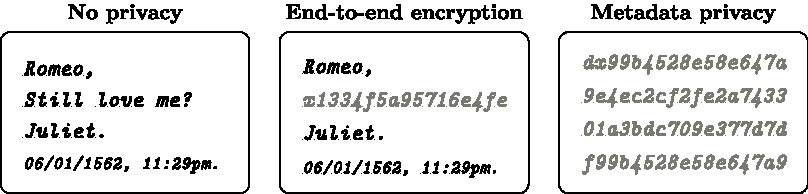
\includegraphics[width=\textwidth]{metadata-privacy.pdf}
\caption{The view of a powerful adversary. With end-to-end encryption, the adversary can still see the metadata.}
\label{fig:metadataprivacy}
\end{figure}

This section describes our desired properties and the threat model we want them to hold in. In short, we guarantee metadata privacy against everyone except the conversation partners themselves.

\subsection{Goals}
%From the start, Anysphere has assumed a few basic goals to guide our work.
% The goals below are in reference to an attacker with the capabilities defined in the threat model section (\cref{subsec:threatmodel}). <- implicit from the section below. Distracts and asks the reader to jump below.

\textbf{1. Metadata privacy.} An attacker cannot learn anything about what messages are being sent when, between whom. This implies that the attacker cannot read messages (because it does not even know that the messages exist). We guarantee one of the strongest possible versions of metadata privacy; for more details, see \cref{subsec:core-security}.
% : formally, an attacker can simulate its view in the real world given only the knowledge of its own messages <- Lets leave this for the formal section. If we cannot explain, it its weird to make this claim here.
% \xxx[sualeh]{It would be awesome to have a clearer sentence for the formal claim. I have not come up with one yet.}

\textbf{2. Integrity.} An attacker cannot forge a message from anyone, or edit any of the messages being sent.

\textbf{3. Resistance to client-side denial-of-service attacks}. An attacker that merely controls some number of users cannot block messages from being delivered. We do not guarantee service against an attacker that controls the server or the network.

\textbf{4. Reasonable load on the client.} Users are able to run a client on any commonly sold internet device. The client load should be adjustable.

\section{Threat Model}

\todo{add table comparing our threat model with e.g. signal and email}
\todo{add an illustration of a walled garden, with the walls containing only your computer and your friends' computers}

%Touch on: server, friends, client-side computer, etc.

\todo{Figure out a better format here. See e.g. Skiff's whitepaper.}



Similar to most PIR schemes(for example \cite{ahmad2021addra}, \textsection 2.2), our threat model assumes a global adversary who can compromise the entire communication infrastructure except for the user's and their friends' client end. In particular, we assume the adversary has control over all the servers, and can observe and manipulate all network traffic.

End-user trust is more subtle matter. In \cite{angel2018s}, Angle, Lazar and Tzialla describes the compromised friend(CF) attack on a general meta-data private messaging system, which shows that perfectly hiding metadata while not trusting the user's friends is computationally prohibitive. In our security model, a user trusts that the devices of themselves and all their friends are uncompromised and running an unmodified copy of anysphere's client-side code. The user assumes that any other end-user device might be compromised.

\todo{Can we assume that only a small number of friends are compromised?}

Finally, we assume the security of the standard cryptography primitives we use, including microsoft SEAL's BFV cryptosystem and libsodium's AEAD cryptosystem. 

Denial of Service(DoS) attacks are unavoidable if the adversary controls all our servers. In the case of such attacks, we do not guarantee liveliness of our service, but continue to guarantee metadata security. We also defend against DoS attacks launched by an end-user with no access to the servers.

\subsection{Desired Properties}

1. \textbf{Perfect Metadata Protection}: All contents and metadatas associated with a conversation are only visible to the users involved with the conversation. Even with a compromised server, an adversary should not even be able to find out whether two users are engaging in any conversation.

2. \textbf{Forward Secrecy}: \todo{do we provide this?}

3. \textbf{Resistant to man-in-the-middle attacks}.

4. \textbf{Resistant to social engineering attacks}.

\todo{add more.}



